\documentclass{standalone}
\usepackage{tikz}
\usepackage{ctex,siunitx}
\setCJKmainfont{Noto Serif CJK SC}
\usepackage{tkz-euclide}
\usepackage{amsmath}
\usepackage{wasysym}
\usetikzlibrary{patterns, calc}
\usetikzlibrary {decorations.pathmorphing, decorations.pathreplacing, decorations.shapes,}
\begin{document}
\small
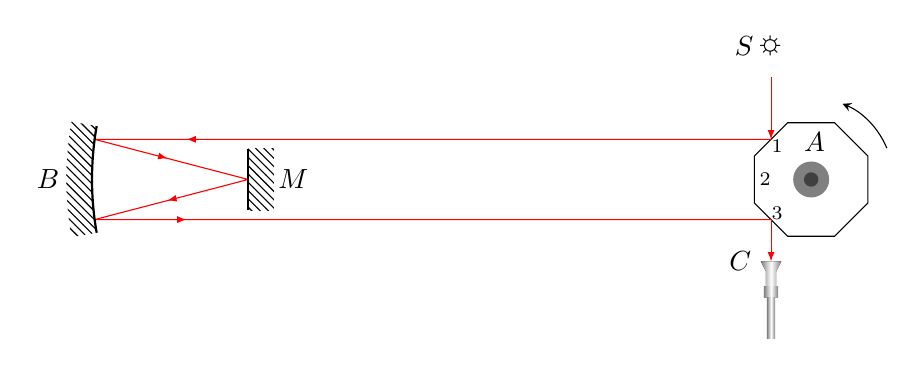
\begin{tikzpicture}[>=stealth,scale=1.3]
  % \useasboundingbox(-2.4,-2.1)rectangle(7.5,2.5);
  \fill[gray](0,0)circle(5pt);
  \fill[darkgray](0,0)circle(2pt);
  \draw(22.5:0.6)--(67.5:0.6)node[below left]{$A$}--(112.5:0.6)--(157.5:0.6)--(202.5:0.6)--(247.5:0.6)--(292.5:0.6)--(-22.5:0.6)--cycle;
  \draw[->](22.5:0.8)arc(22.5:67.5:0.8);
  \node at (-0.392,1.3){\sun};
  \node at (-0.392,1.3)[left=1mm]{$S$};
  \draw[line join=round,red,postaction={decorate},decoration={markings,mark={between positions 0.35 and 0.7 step 0.1 with {\arrow{Latex[scale=0.7]}}}}] (-0.392,0.392)node[inner sep=0pt,below right,text=black]{\scriptsize 1}--(-7,0.392)--(-5.5,0)--(-7,-0.392)--(-0.392,-0.392)node[inner sep=0pt,above right,text=black]{\scriptsize 3};
  \node at (-0.6,0)[right]{\scriptsize 2};
  \draw[red,arrows={-Latex[scale=0.7]}](-0.392,-0.392)--(-0.392,-0.8);
  \draw[red,arrows={-Latex[scale=0.7]}](-0.392,1.0)--(-0.392,0.392);
  \draw[thick](-6.9801,0.5215)arc(170:190:3);
  \fill[pattern=north west lines](-6.9801,0.5215)arc(170:190:3)--++(190:0.25)arc(190:170:3.25)--cycle;
  \draw[thick](-5.5,0.3)--(-5.5,-0.3);
  \fill[pattern=north west lines](-5.5,0.3)rectangle(-5.25,-0.3);
  \begin{scope}[xshift=-0.392cm,yshift=-0.8cm]
    \node at (-0.1,0)[left]{$C$};
  \fill[left color=gray,right color=gray, middle color=white](-0.1,0)--(0.1,0)--(0.05,-0.1)--(-0.05,-0.1)(-0.05,-0.1)rectangle(0.05,-0.25);
  \fill[left color=gray,right color=gray, middle color=white](-0.07,-0.25)rectangle(0.07,-0.35);
  \fill[left color=gray,right color=gray, middle color=white](-0.04,-0.35)rectangle(0.04,-0.75);
  \end{scope}
  \node at (-7.25,0)[left]{$B$};
  \node at (-5.3,0)[right]{$M$};
  
\end{tikzpicture}
\end{document}